\documentclass[12pt]{article}

%packages
\usepackage{fancyhdr}
\usepackage[margin=1in]{geometry}
\usepackage[utf8]{inputenc}
\usepackage{listings}
\usepackage{booktabs}
\usepackage{enumitem}
\usepackage{pdfpages}
\usepackage{graphicx}
\usepackage{listings}
\usepackage{xcolor}
\usepackage{subcaption}
\usepackage{float}
\usepackage{amsmath}

%fancyheadr fix
\setlength{\headheight}{15pt}

%commands to lslistings
\lstset{
    basicstyle=\ttfamily\small,
    breaklines=true,     
    breakatwhitespace=true,
    frame=single,
    numbers=left,
    numberstyle=\tiny,
    columns=fullflexible,
    keepspaces=true
}


%title info
\newcommand{\doctitle}{STA 5635 HW 4}
\newcommand{\name}{Palmer Swanson}
\newcommand{\docdate}{\today}


%document
\begin{document}

\begin{center}
    {\Large \textbf{\doctitle}}\\[6pt]
    {\name}\\[3pt]
    {\docdate}
\end{center}
\vspace{12pt}

\section*{Problem 1}
TISP variable selection method ith threshold operator:
\[
\Theta(x,\lambda,\eta) = 
\begin{cases} 
    0 & \text{if} |x|\leq \lambda \\
    \frac{x}{1+\eta} & |x| > \lambda
\end{cases}
\]
Penalized logistic regression:
\[
L(\boldsymbol{\omega}) = \frac{1}{N}\sum_{j=1}^{N}\text{ln}
(1+e^{-y_j^{*}\boldsymbol{\omega}^T\boldsymbol{x}_j}) + \lambda\sum_{i=1}^{p}p(\omega_i)
\]
assuming \(y_j^*\in \{-1,1\}\)
and algorithm iteration:
\[
\boldsymbol{\omega}^{t+1} = \Theta\left(\boldsymbol{\omega}^{t} + 
\eta'X^T\left[\boldsymbol{y}- \frac{1}{1 + e^{-X\boldsymbol{\omega}^{t}}}\right], \lambda\right)
\]
assuming \(y_j\in \{-0,1\}\).

For \(\eta=0\) and 100 iterations, the first portion of question 1 is shown in Figure \ref{fig:Gisette_portion}:
\begin{figure}[htbp]
    \centering
    \begin{subfigure}{0.48\textwidth}
        \centering
        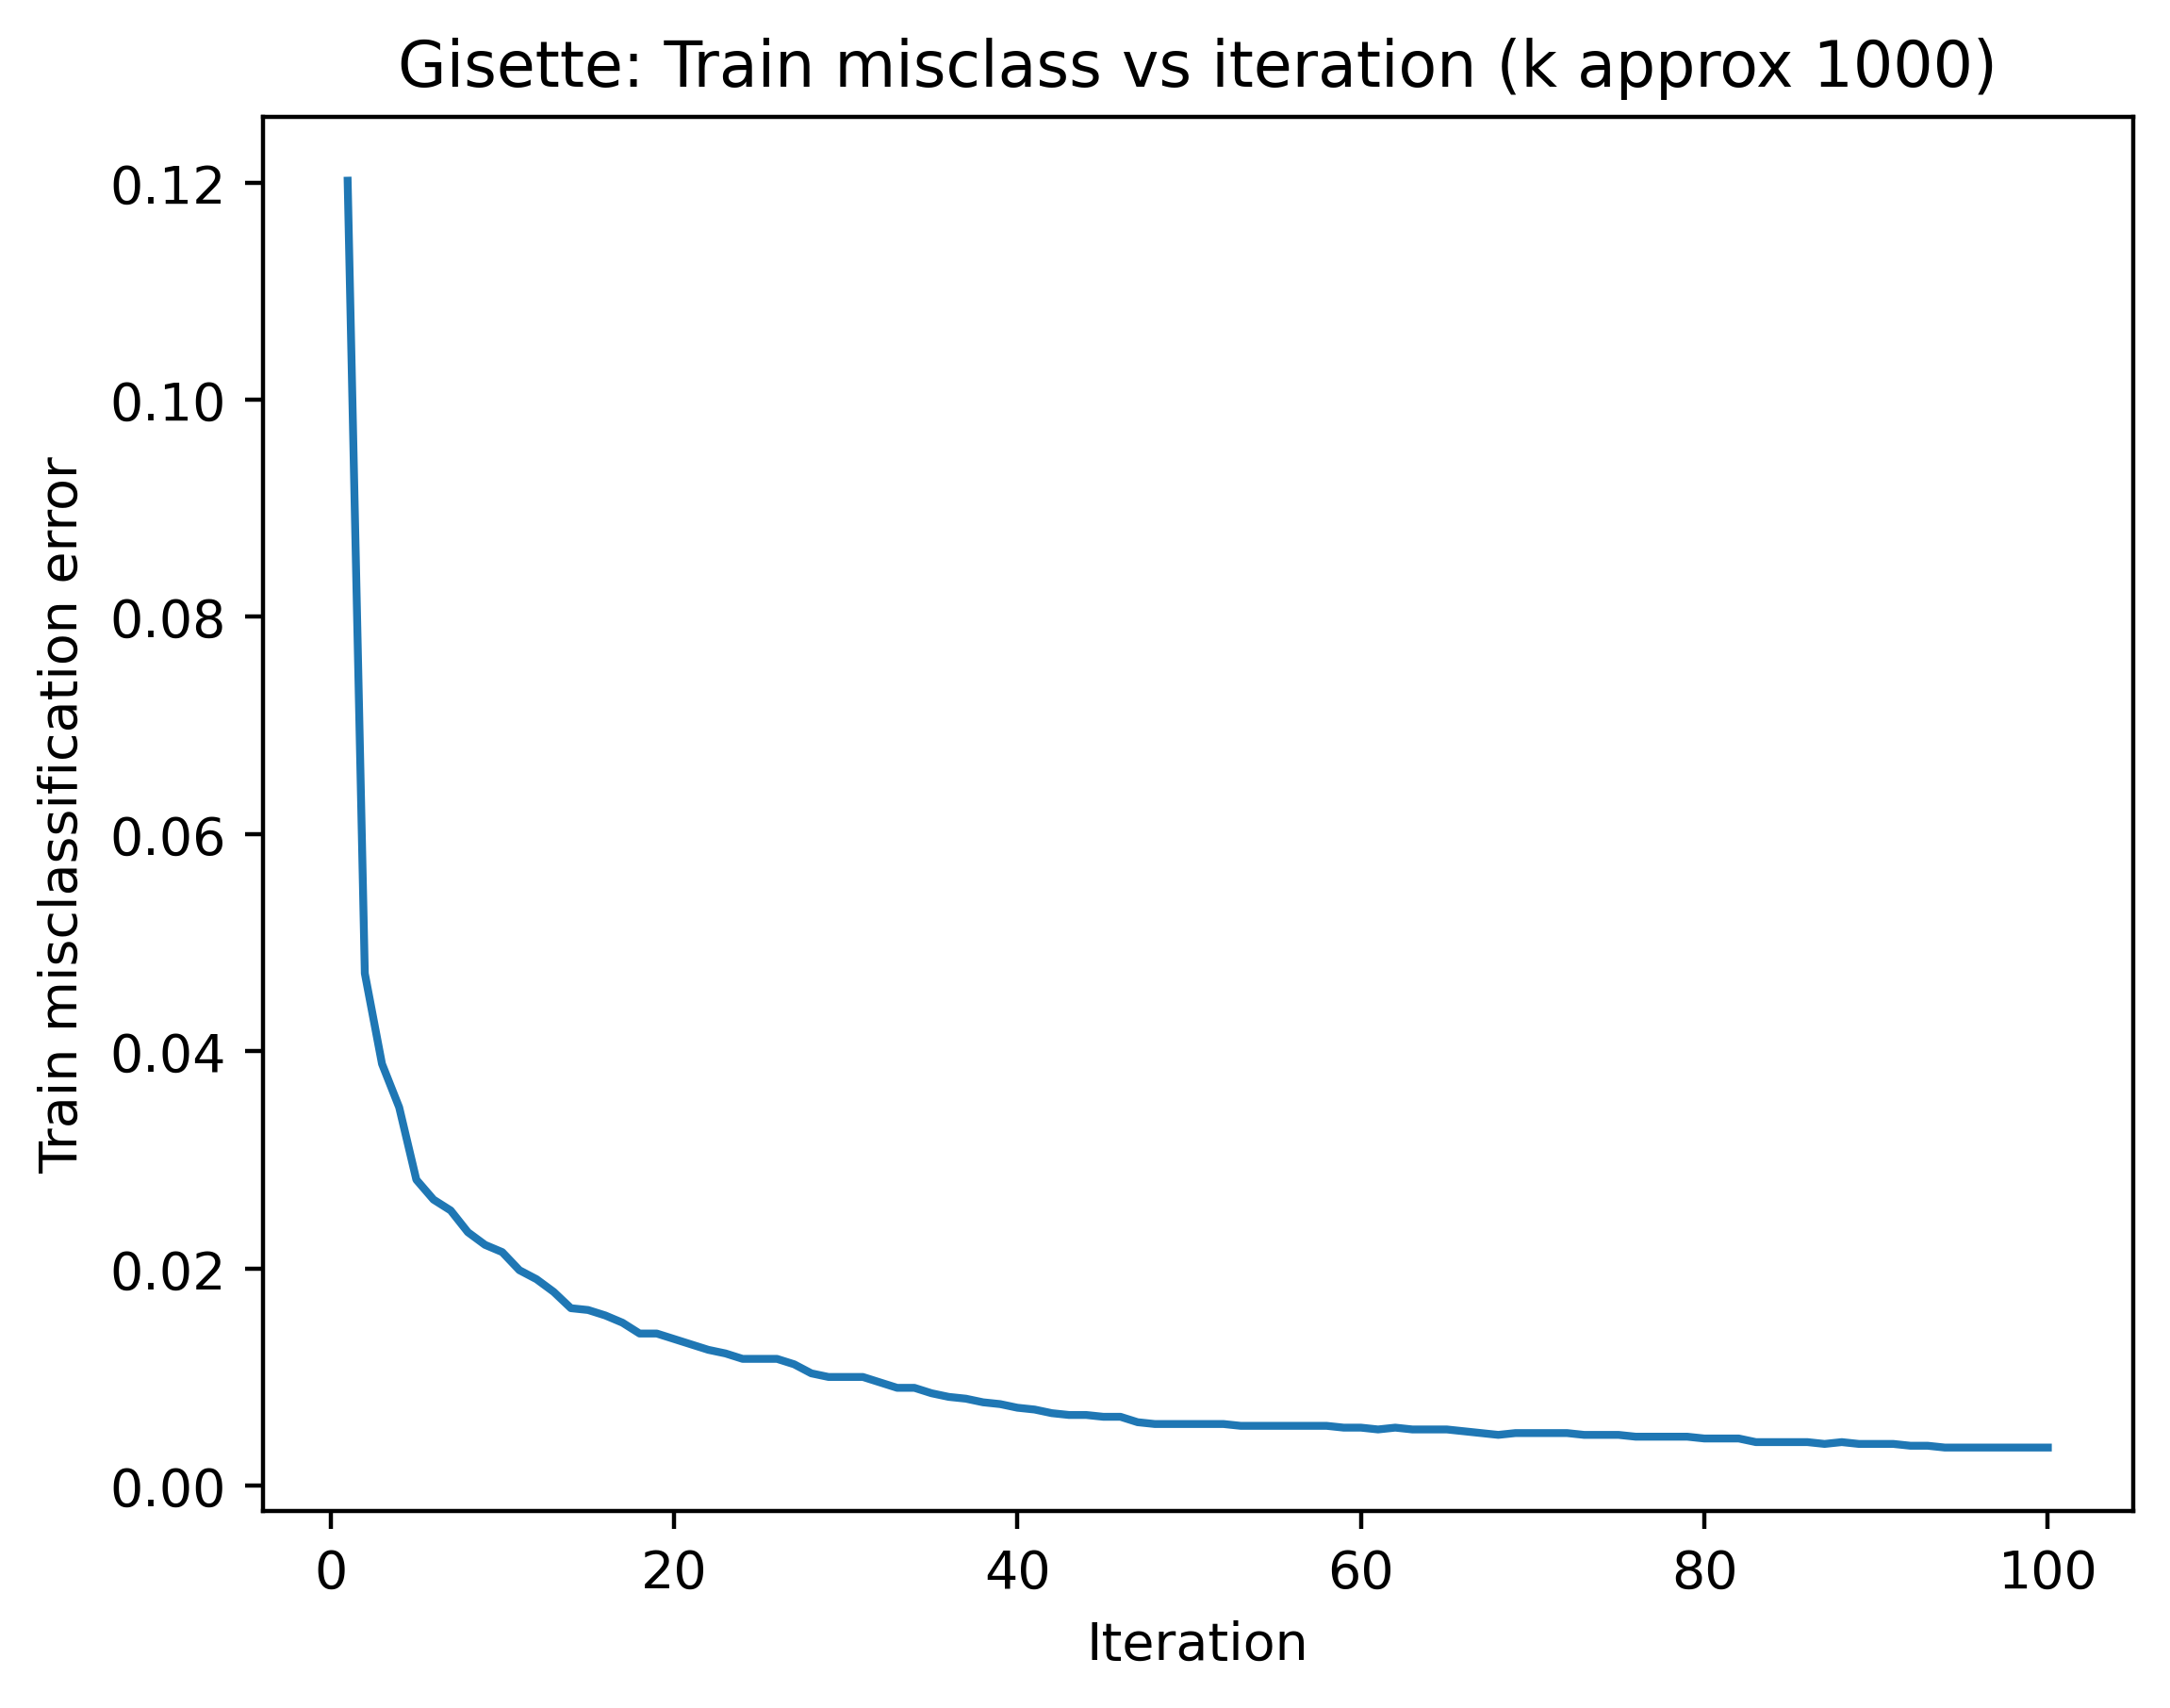
\includegraphics[width=\linewidth]{../figures/gisette_misclass_1000.png}
        \caption{Training misclassification error vs Iteration Number}
    \end{subfigure}
    \hfill
    \begin{subfigure}{0.48\textwidth}
        \centering
        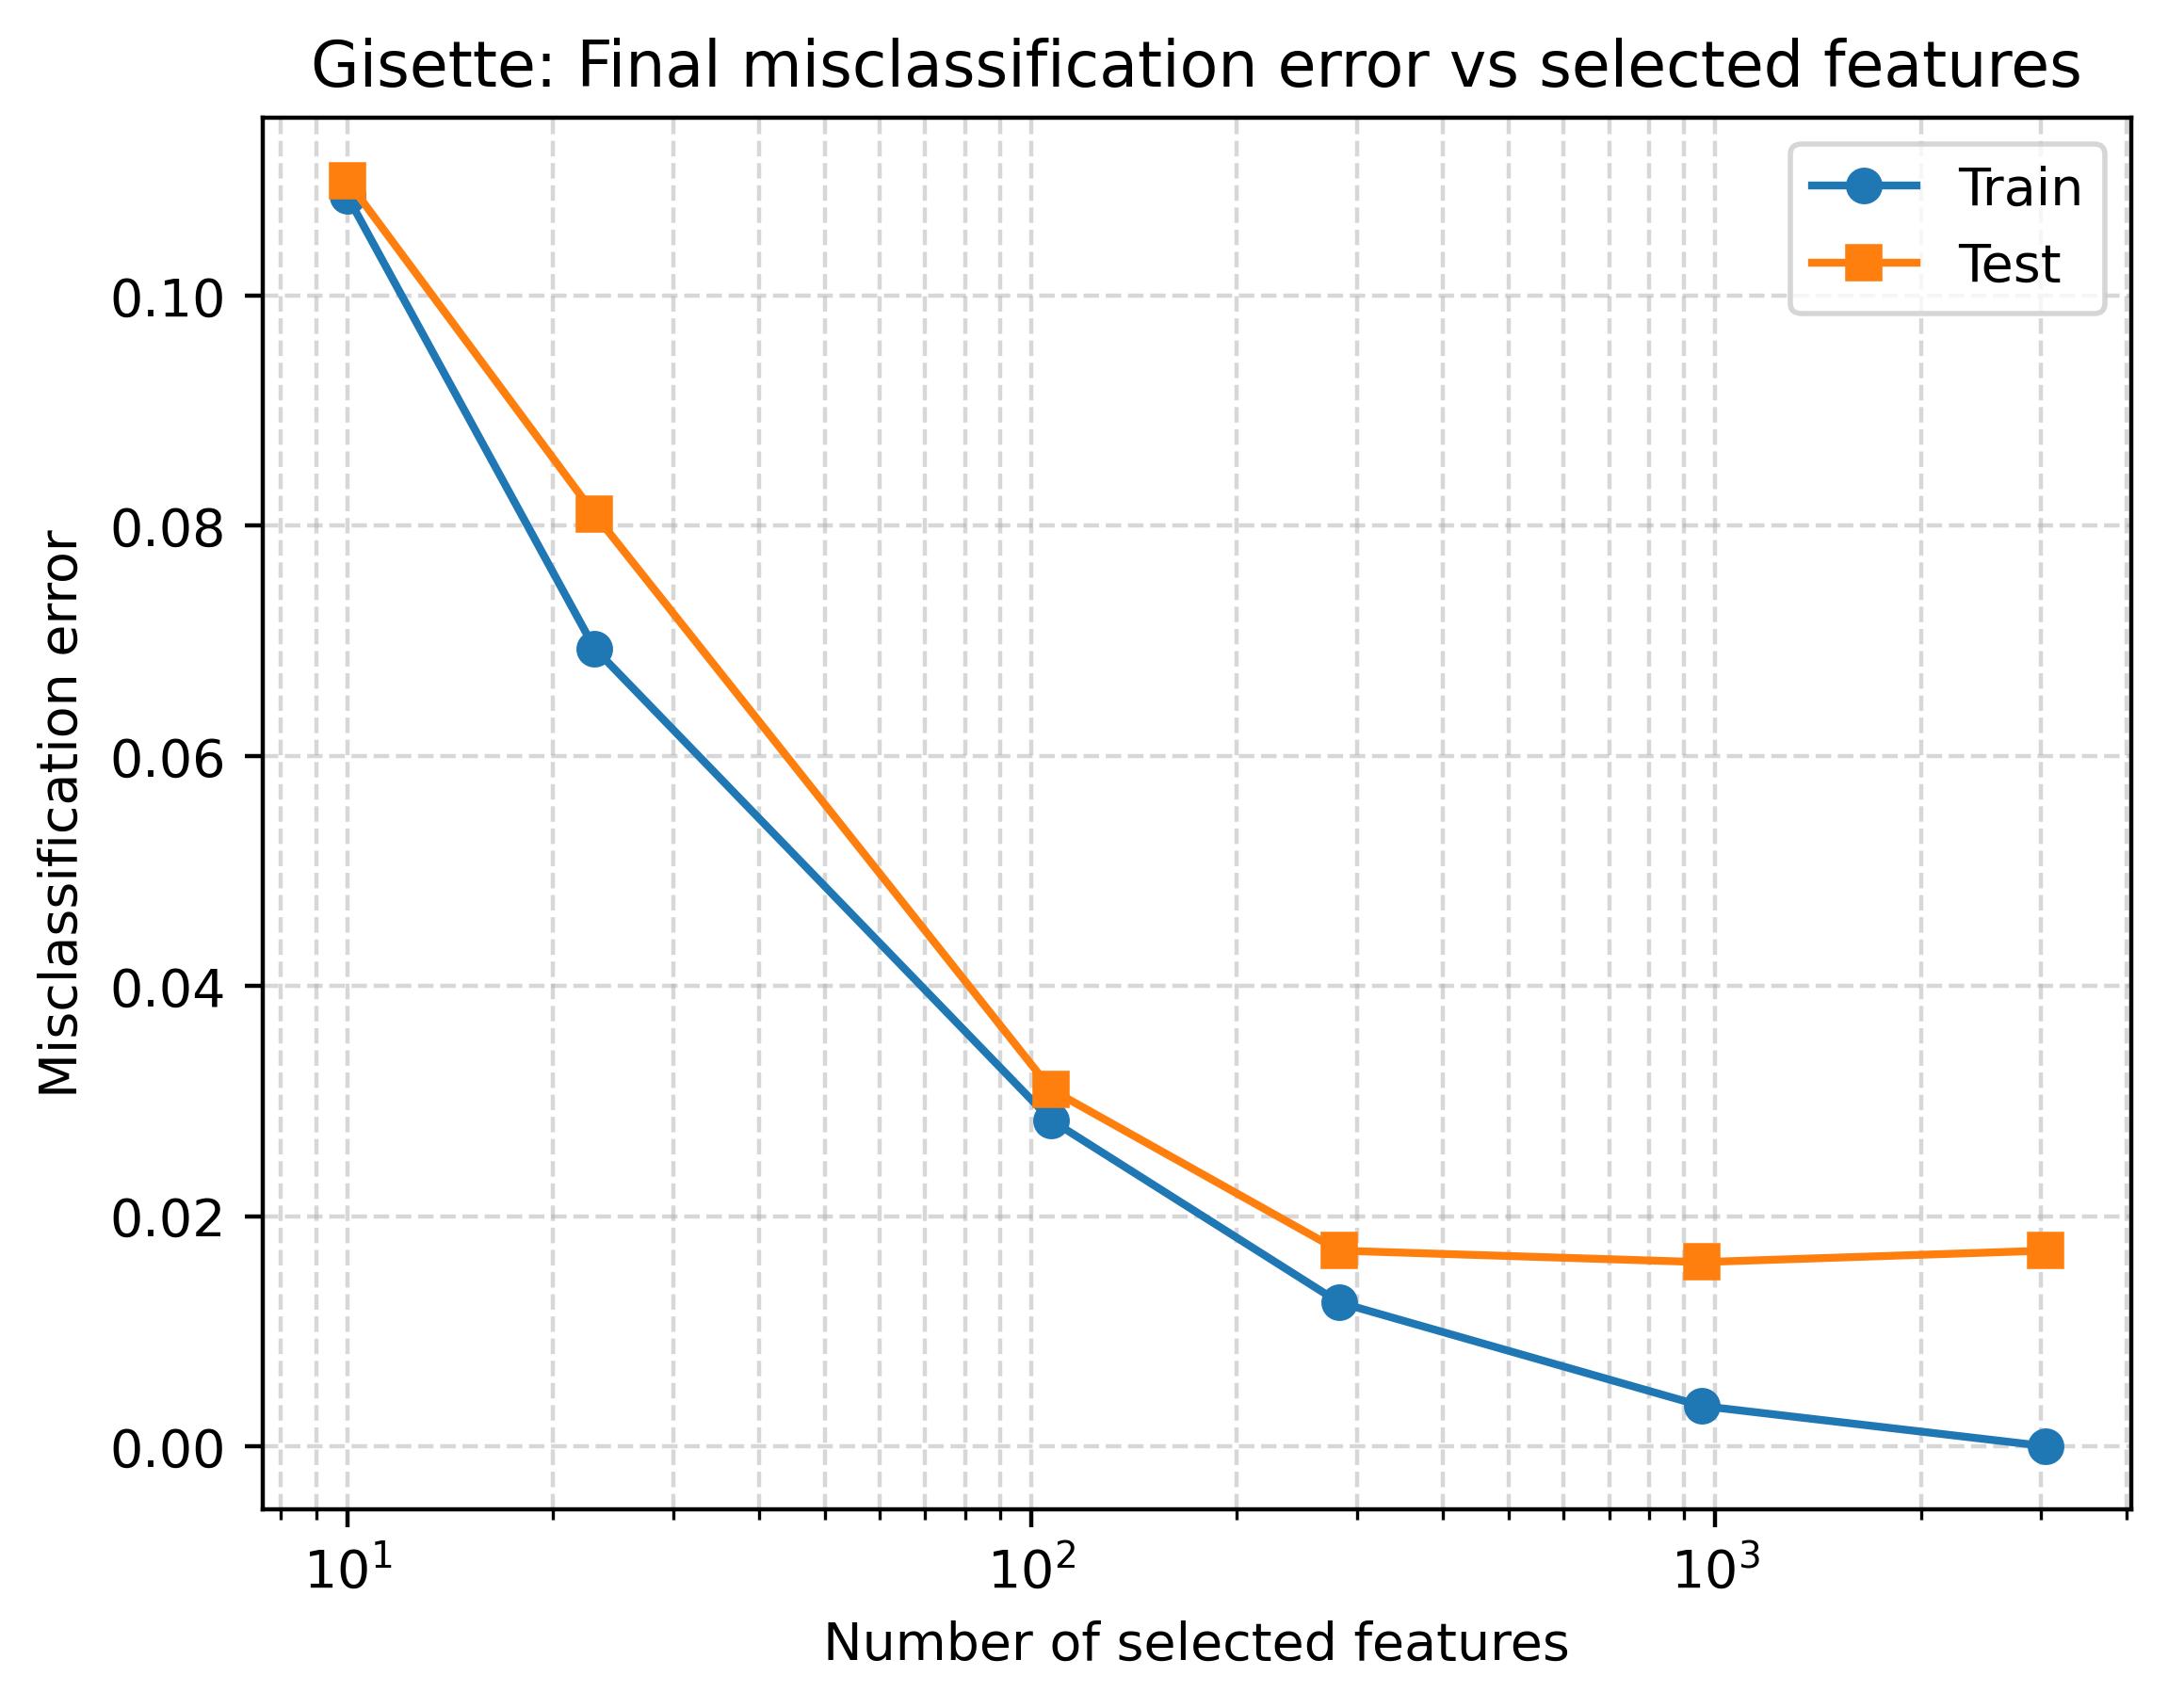
\includegraphics[width=\linewidth]{../figures/Gisette_misclass_vs_features.png}
        \caption{Train and Test Misclassification error vs Number of Selected Features}
    \end{subfigure}
    \caption{Train Misclassification Error vs. TISP iteration (left) and Train and Test Misclassification 
    Error vs. Number of Selected Features (right).  Gisette Dataset.}
    \label{fig:Gisette_portion}
\end{figure}

Second portion of question 1 is hown in Figure \ref{fig:Dexter_portion}
\begin{figure}[htbp]
    \centering
    \begin{subfigure}{0.48\textwidth}
        \centering
        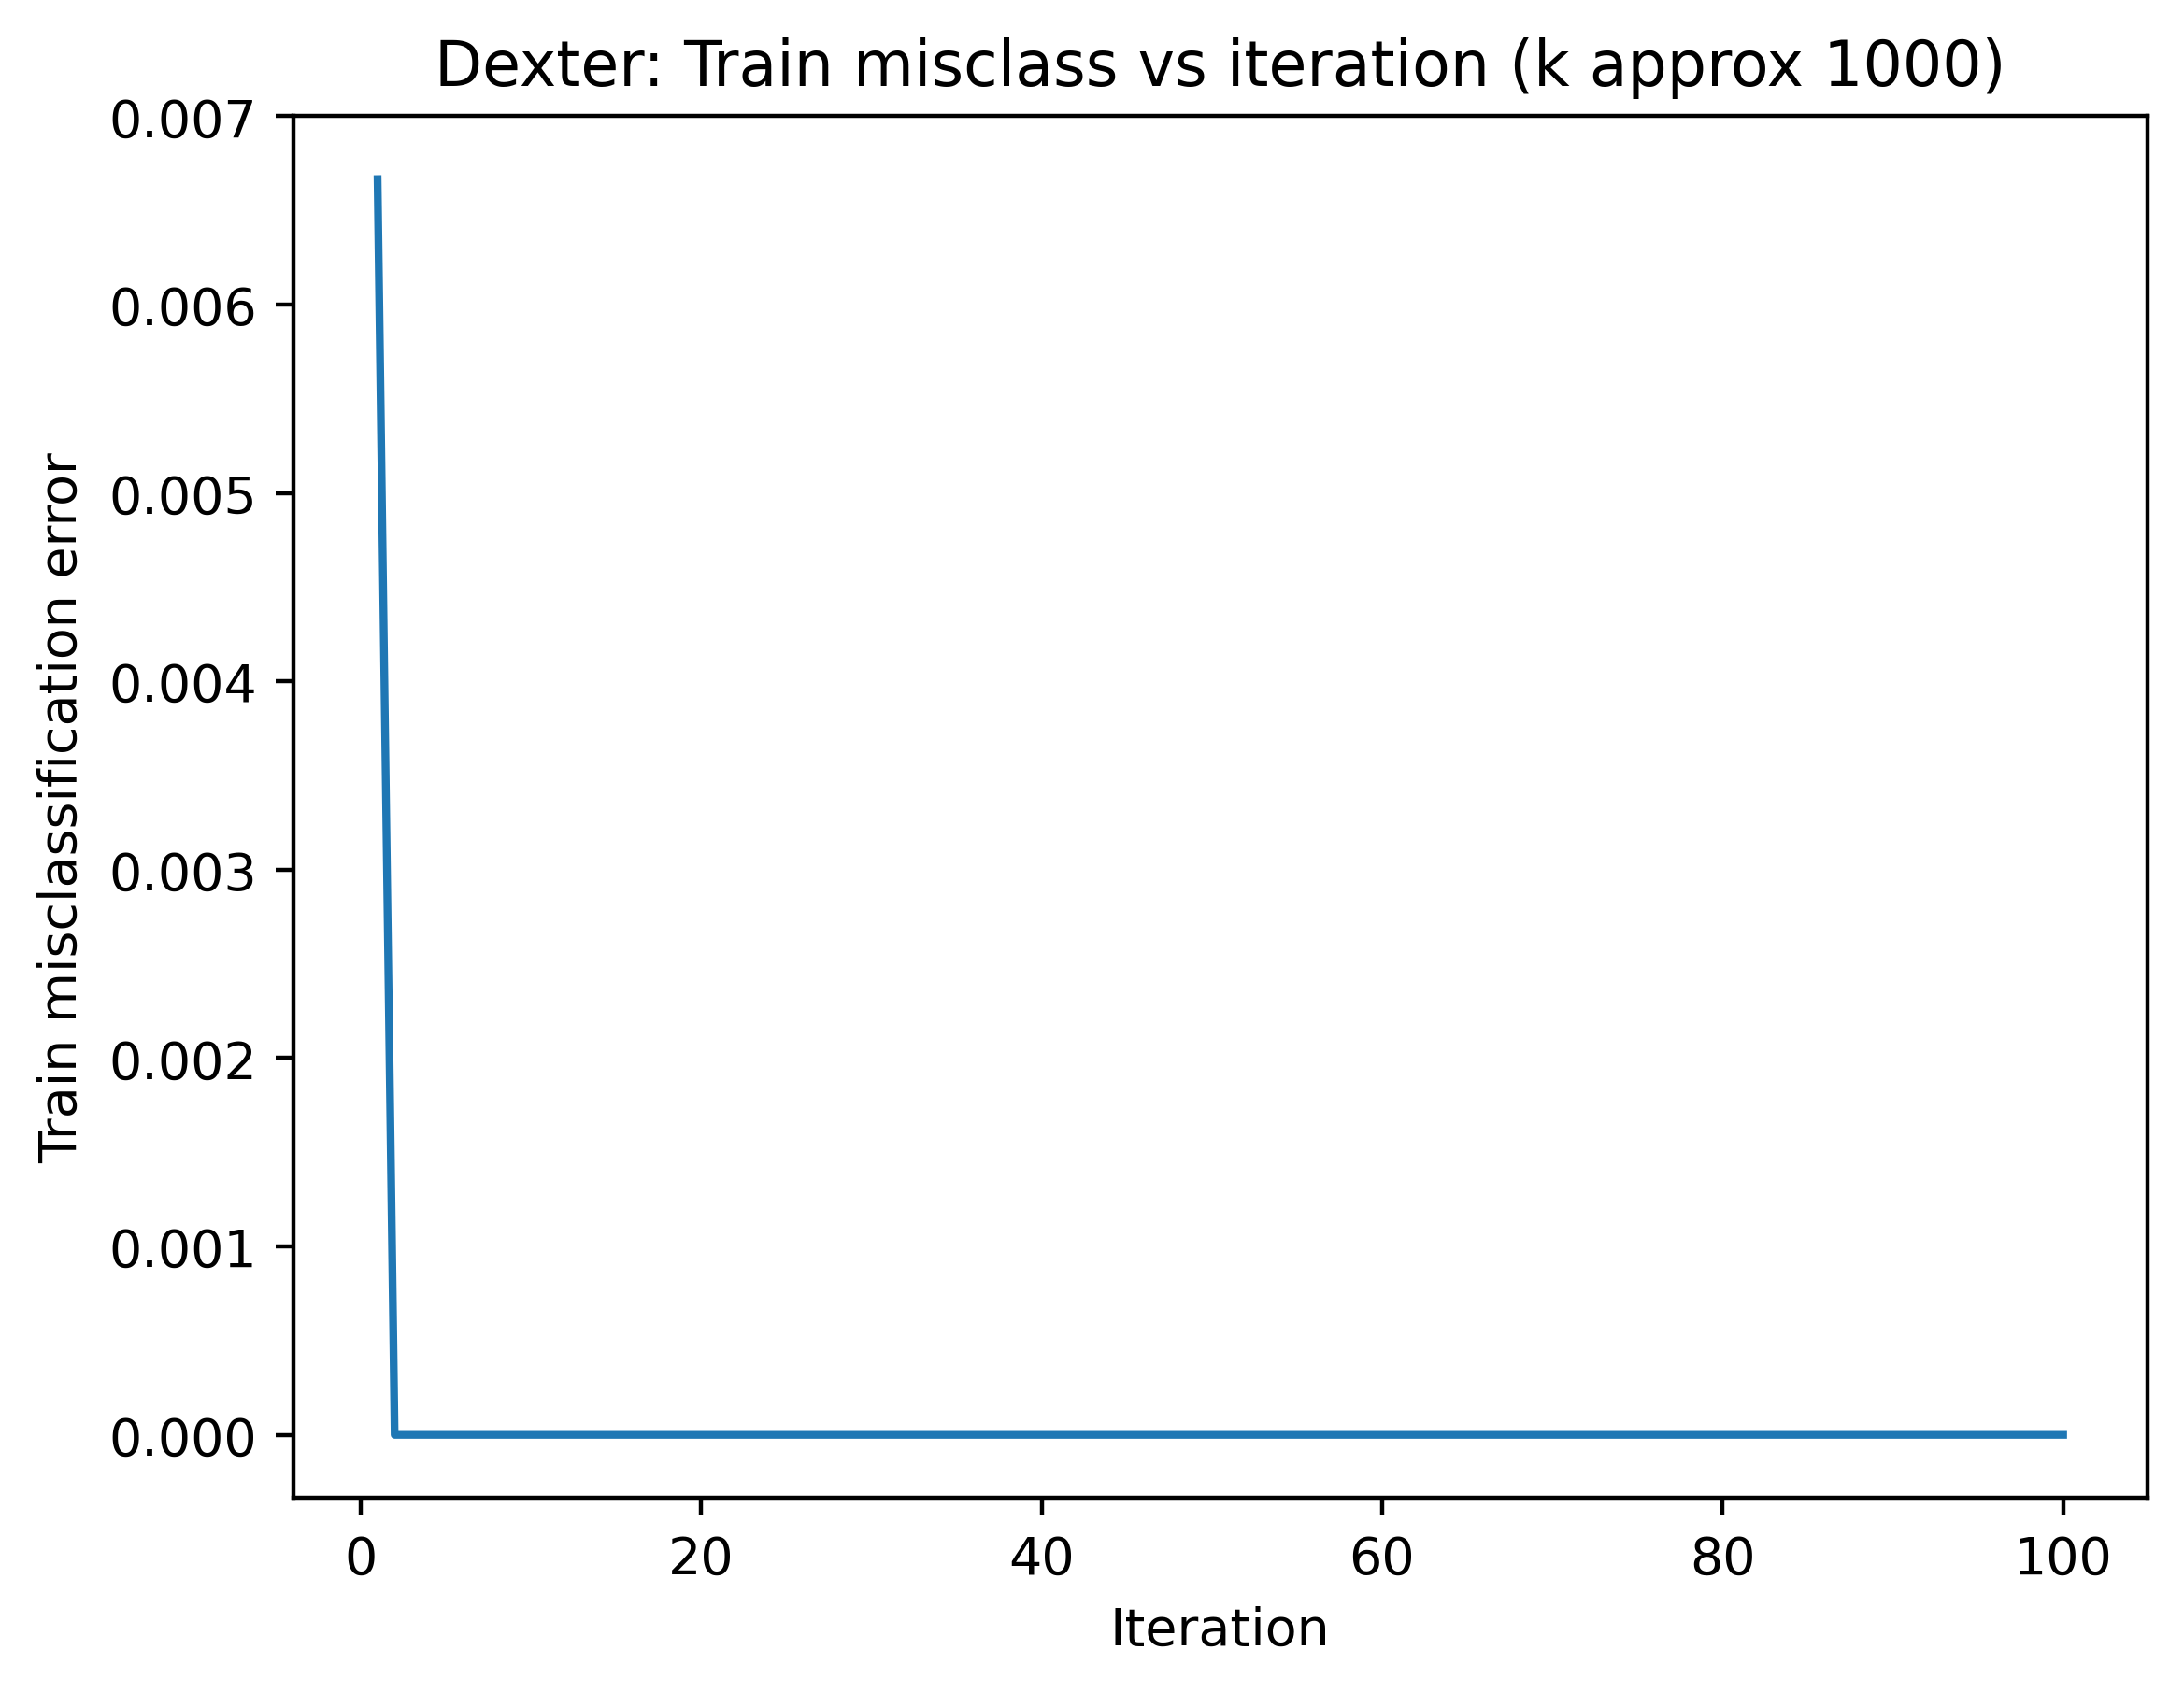
\includegraphics[width=\linewidth]{../figures/dexter_misclass_1000.png}
        \caption{Training misclassification error vs Iteration Number}
    \end{subfigure}
    \hfill
    \begin{subfigure}{0.48\textwidth}
        \centering
        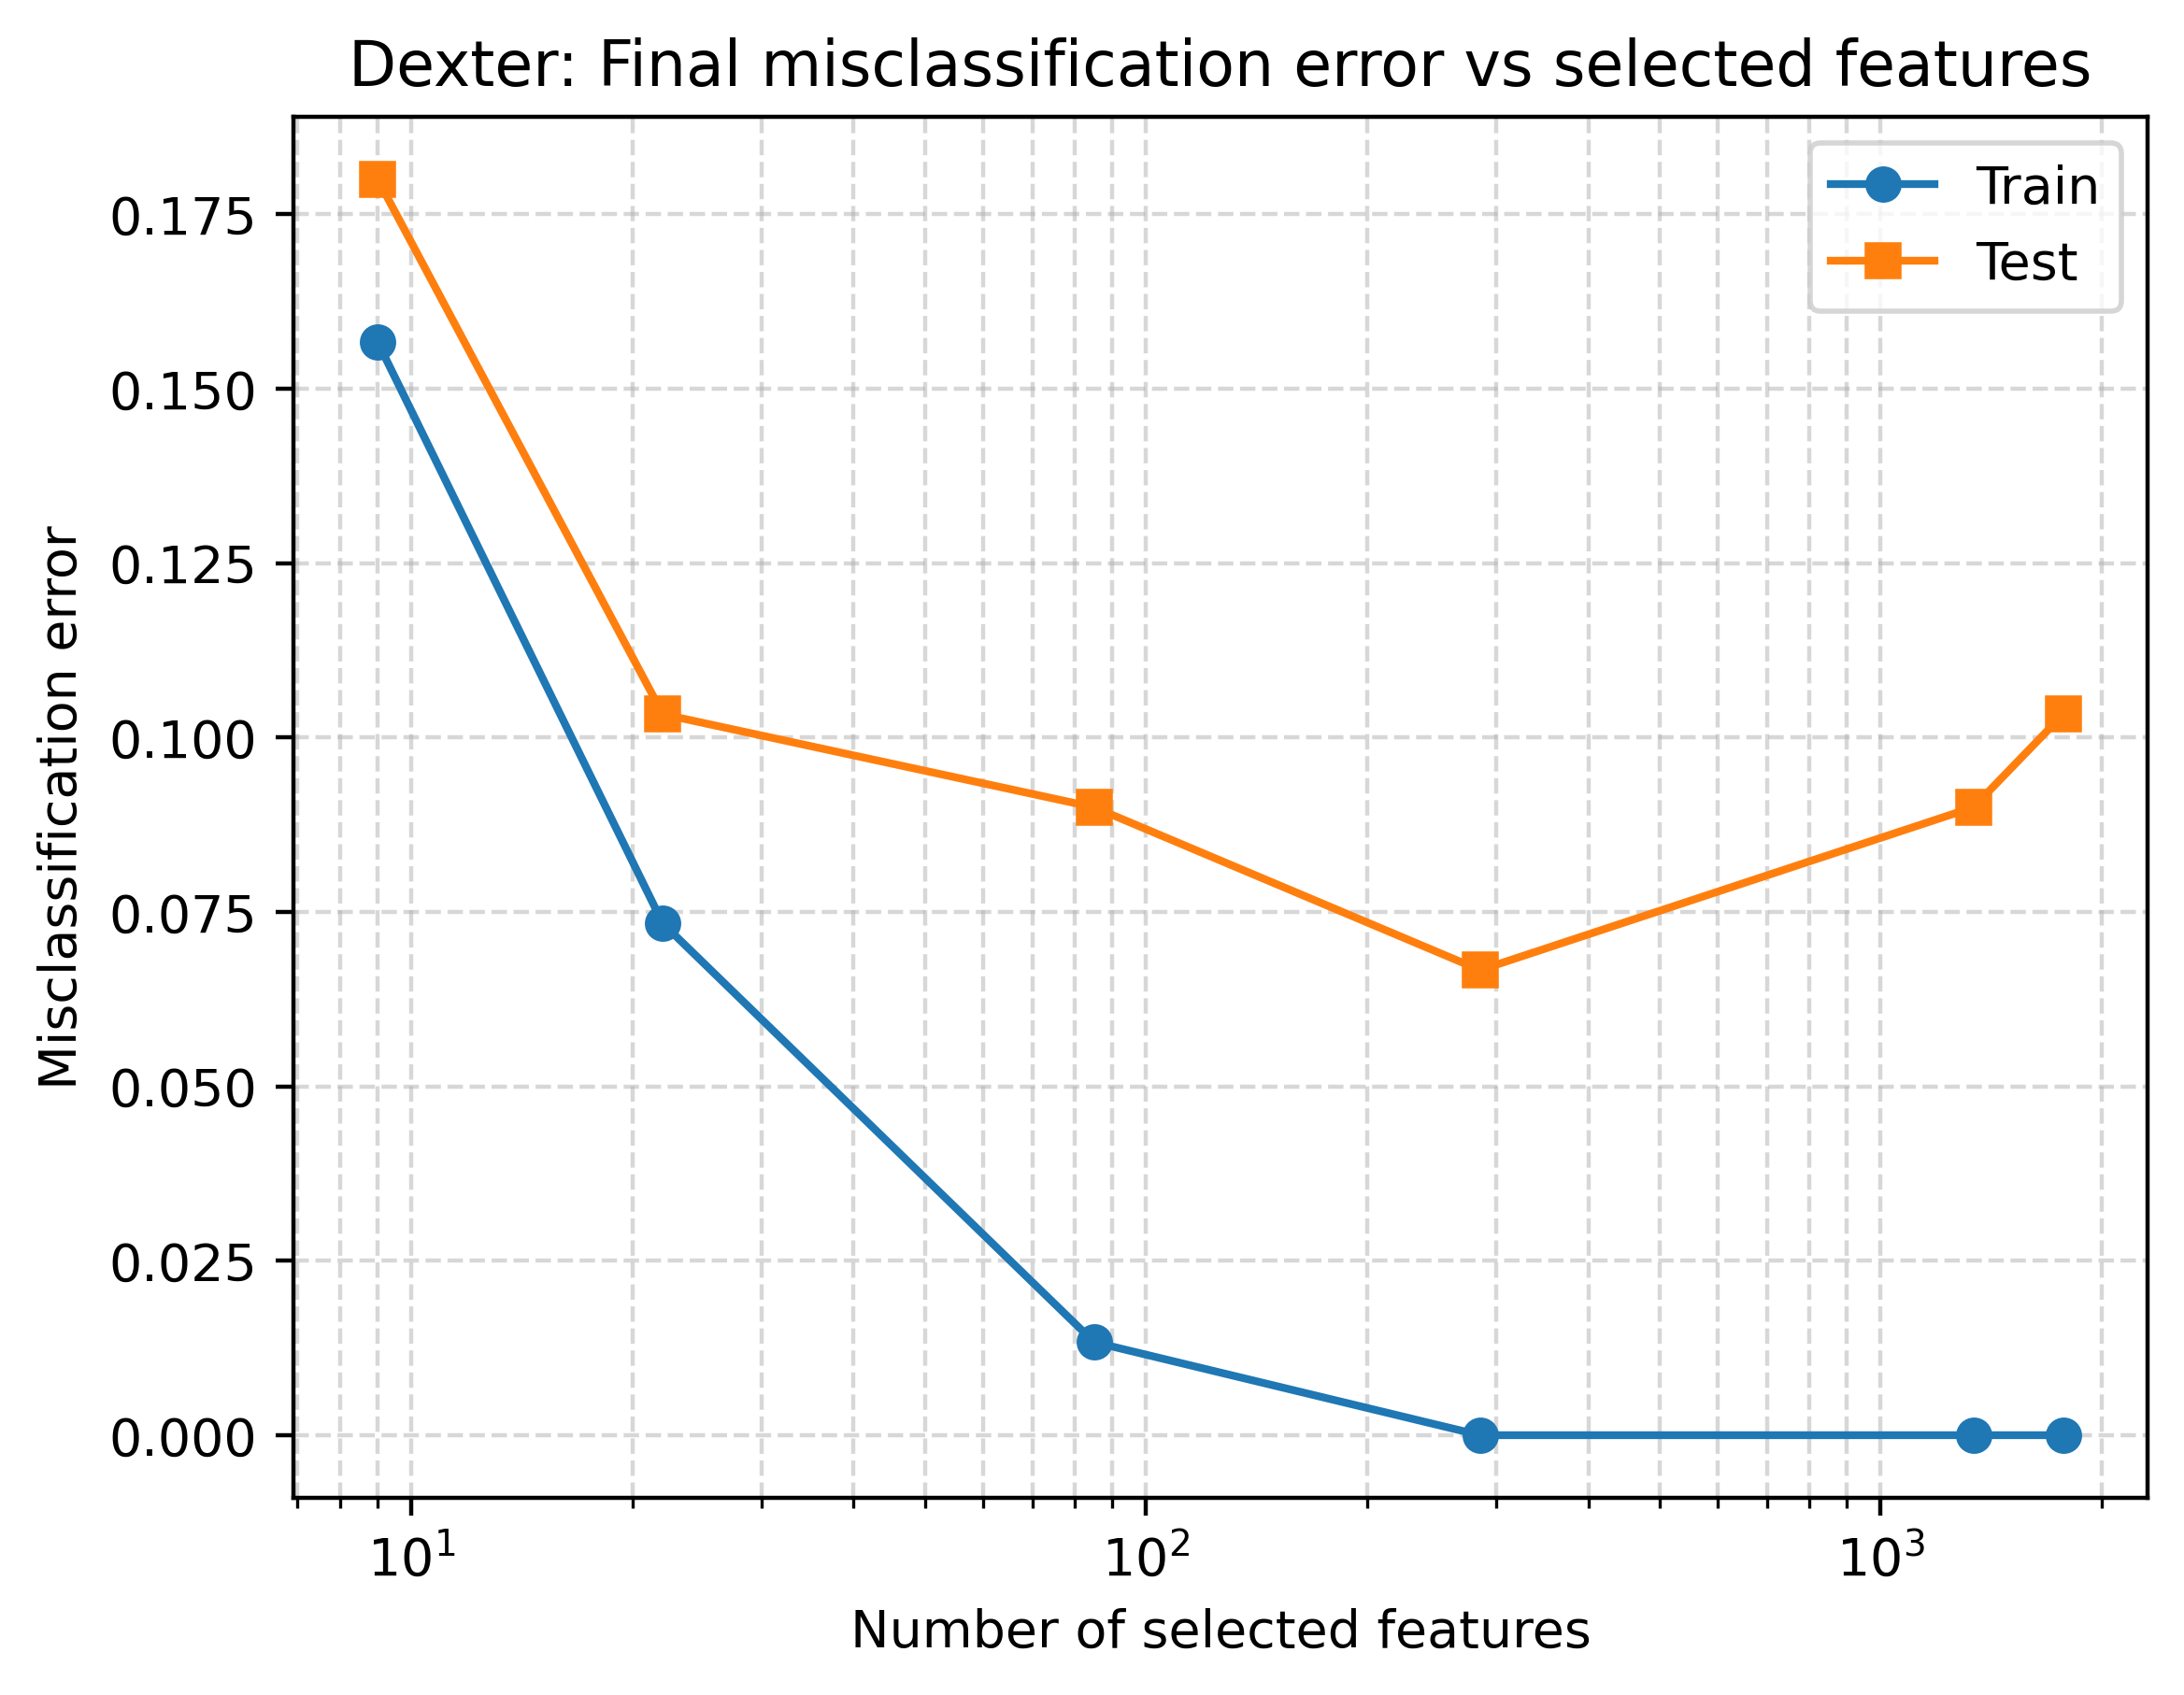
\includegraphics[width=\linewidth]{../figures/Dexter_misclass_vs_features.png}
        \caption{Train and Test Misclassification error vs Number of Selected Features}
    \end{subfigure}
    \caption{Train Misclassification Error vs. TISP iteration (left) and Train and Test Misclassification 
    Error vs. Number of Selected Features (right).  Dexter Dataset.}
    \label{fig:Dexter_portion}
\end{figure}

The table reporting the train and test misclassification error, the test AUC, corresponding number of features
selected, values of \(\lambda\), and the training time are reported in

 \begin{table}[htbp]
    \centering
    \resizebox{\textwidth}{!}{
        \input{../output/misclass_table.tex}
    }
    \caption{Train and Test Misclassification Errors, Test AUC, Number of Selected Features, values of 
    \(\lambda\), and training time, TISP algorithm.}
    \label{tab:table_q1}
\end{table}

\section*{Problem 2}
FSA variable selection using logistic loss with shrinkage:
\[
L_D(\beta) = \frac{1}{N}\sum_{i=1}^{N}\text{ln}
(1+e^{-y_i\beta^T\boldsymbol{x}_j}) + s\lVert\beta\rVert_{2}^{2}
\]
Inverse scheduler with parameter \(\mu\):
\[
M_i = k + (p-k)\text{max}\left(0, \frac{N^{iter}-2i}{2i\mu+N^{iter}}\right)
\]
For \(s=0.001\), \(\mu=100\), and 100 iterations, the first portion of question 2 is shown in

\begin{figure}[htbp]
    \centering
    \begin{subfigure}{0.48\textwidth}
        \centering
        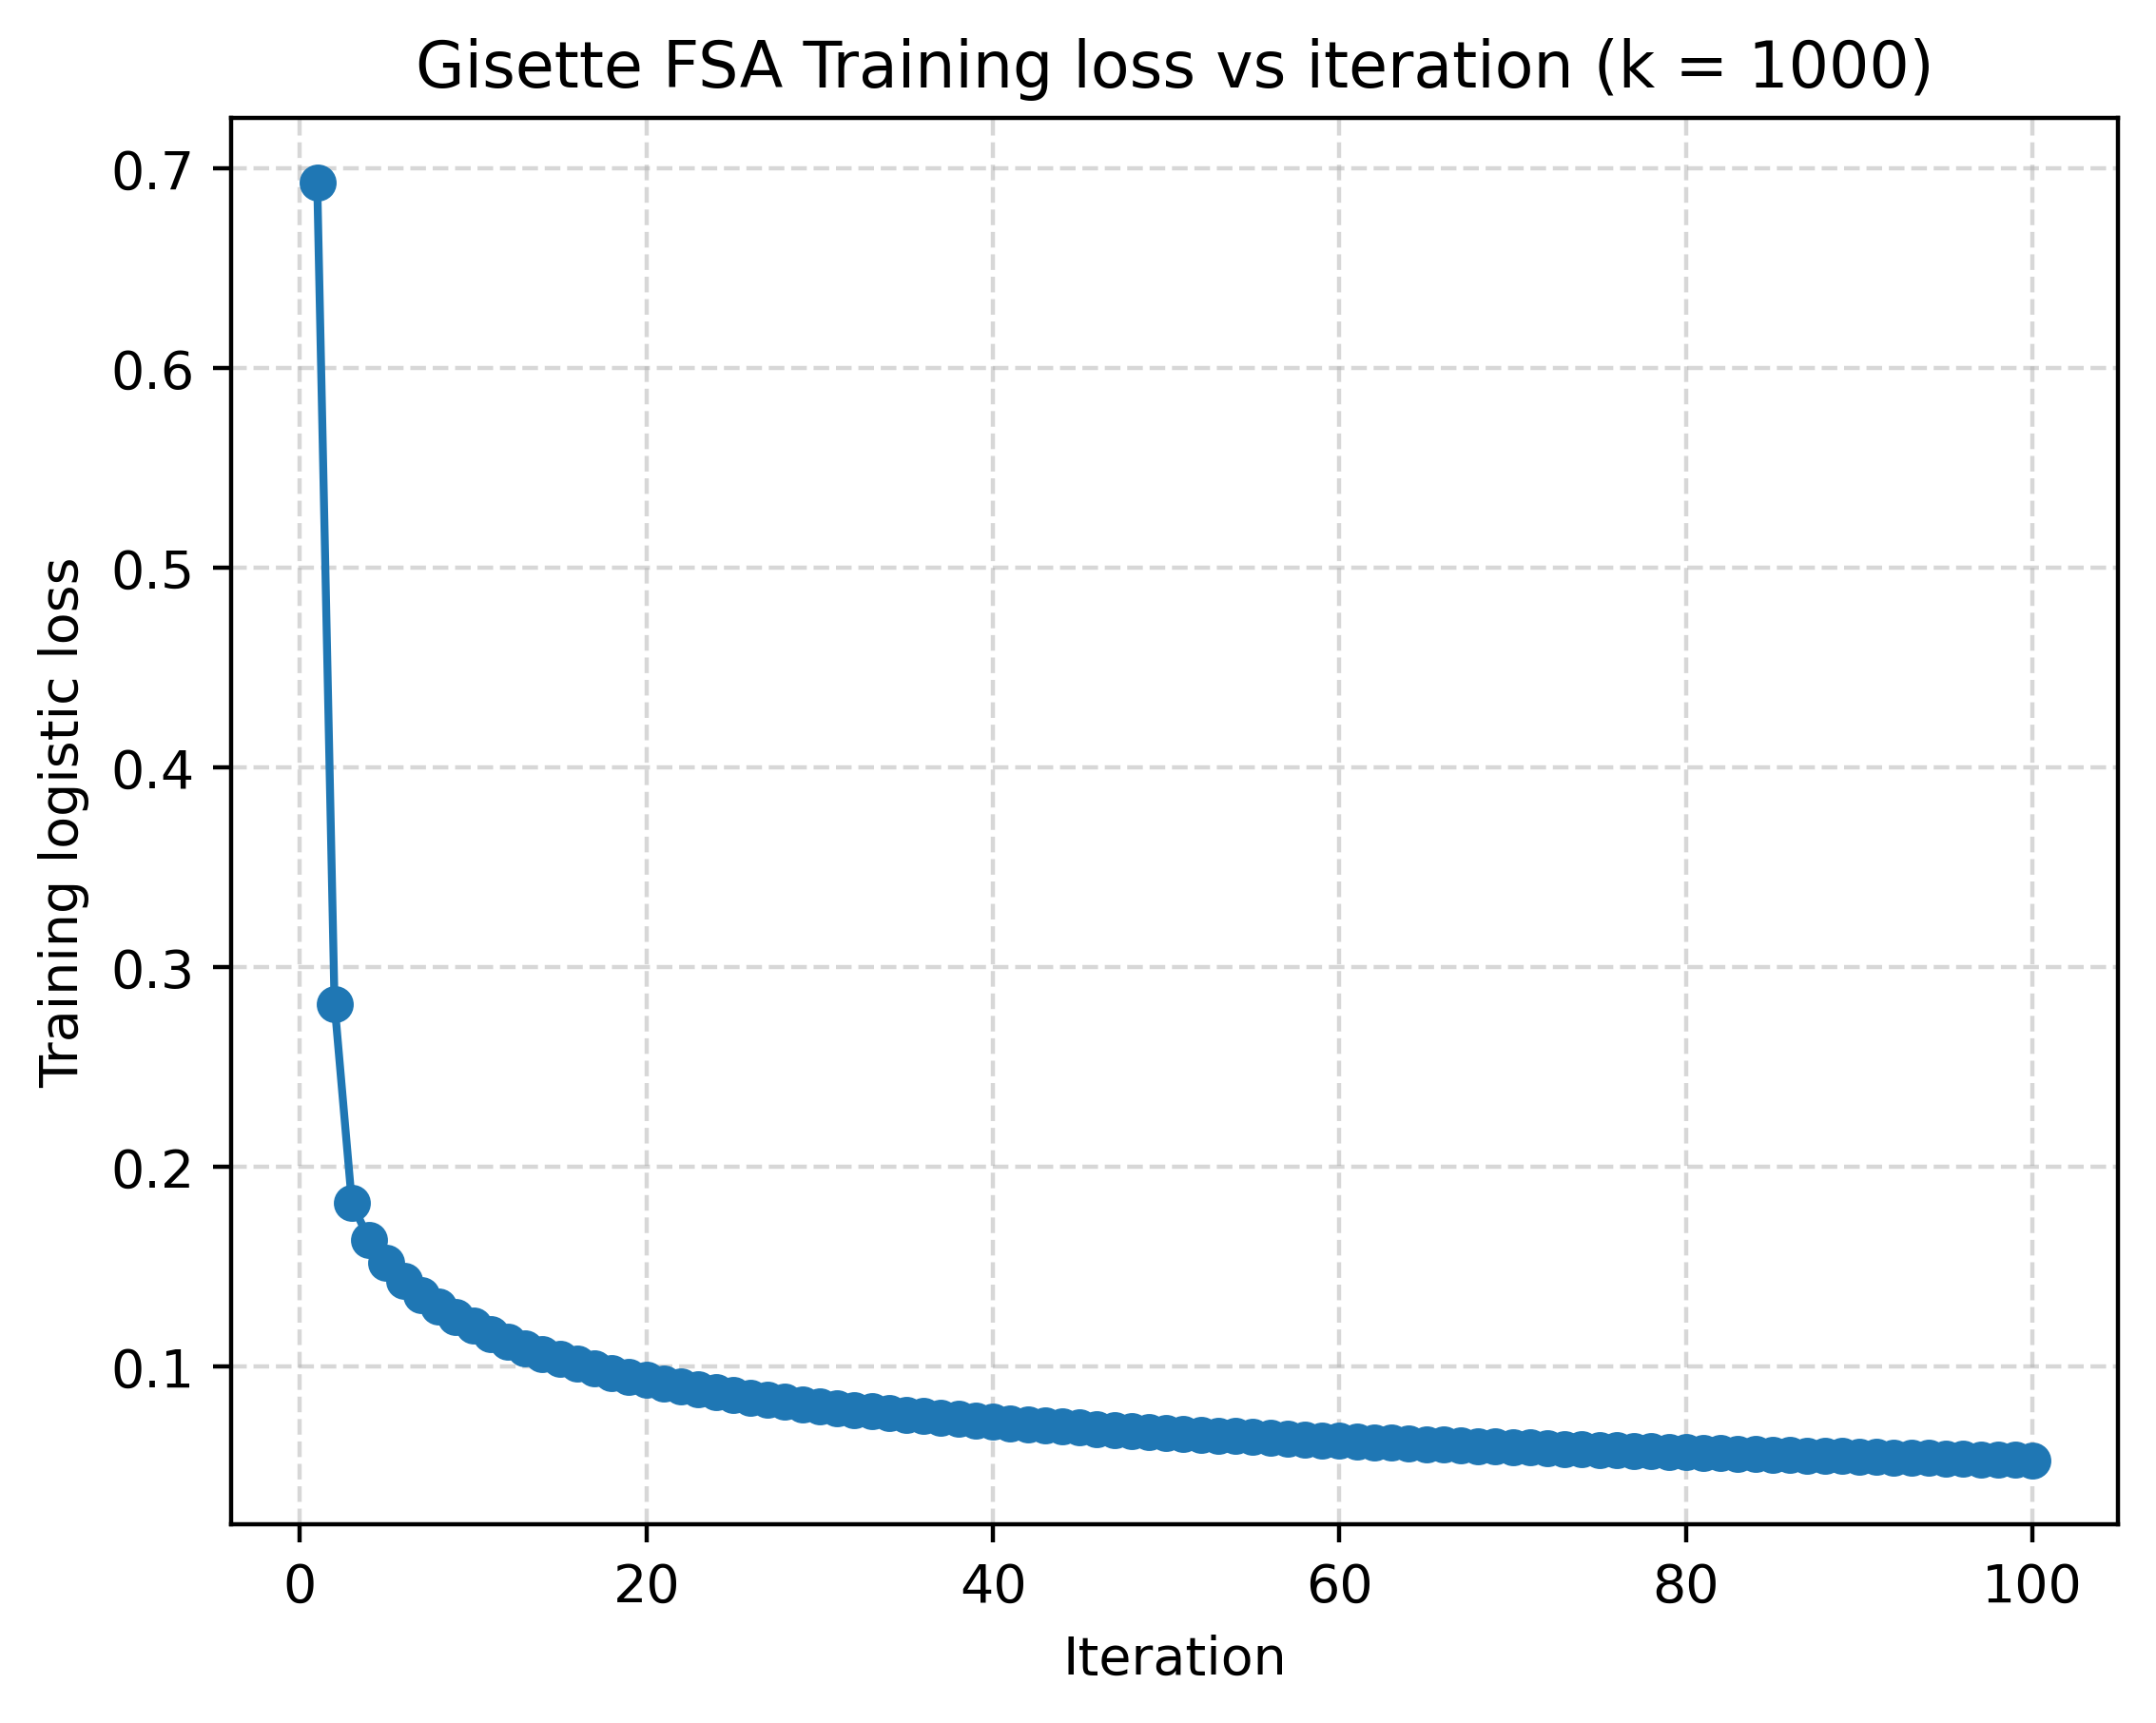
\includegraphics[width=\linewidth]{../figures/gisette_misclass_1000_FSA.png}
        \caption{Gisette Dataset}
    \end{subfigure}
    \hfill
    \begin{subfigure}{0.48\textwidth}
        \centering
        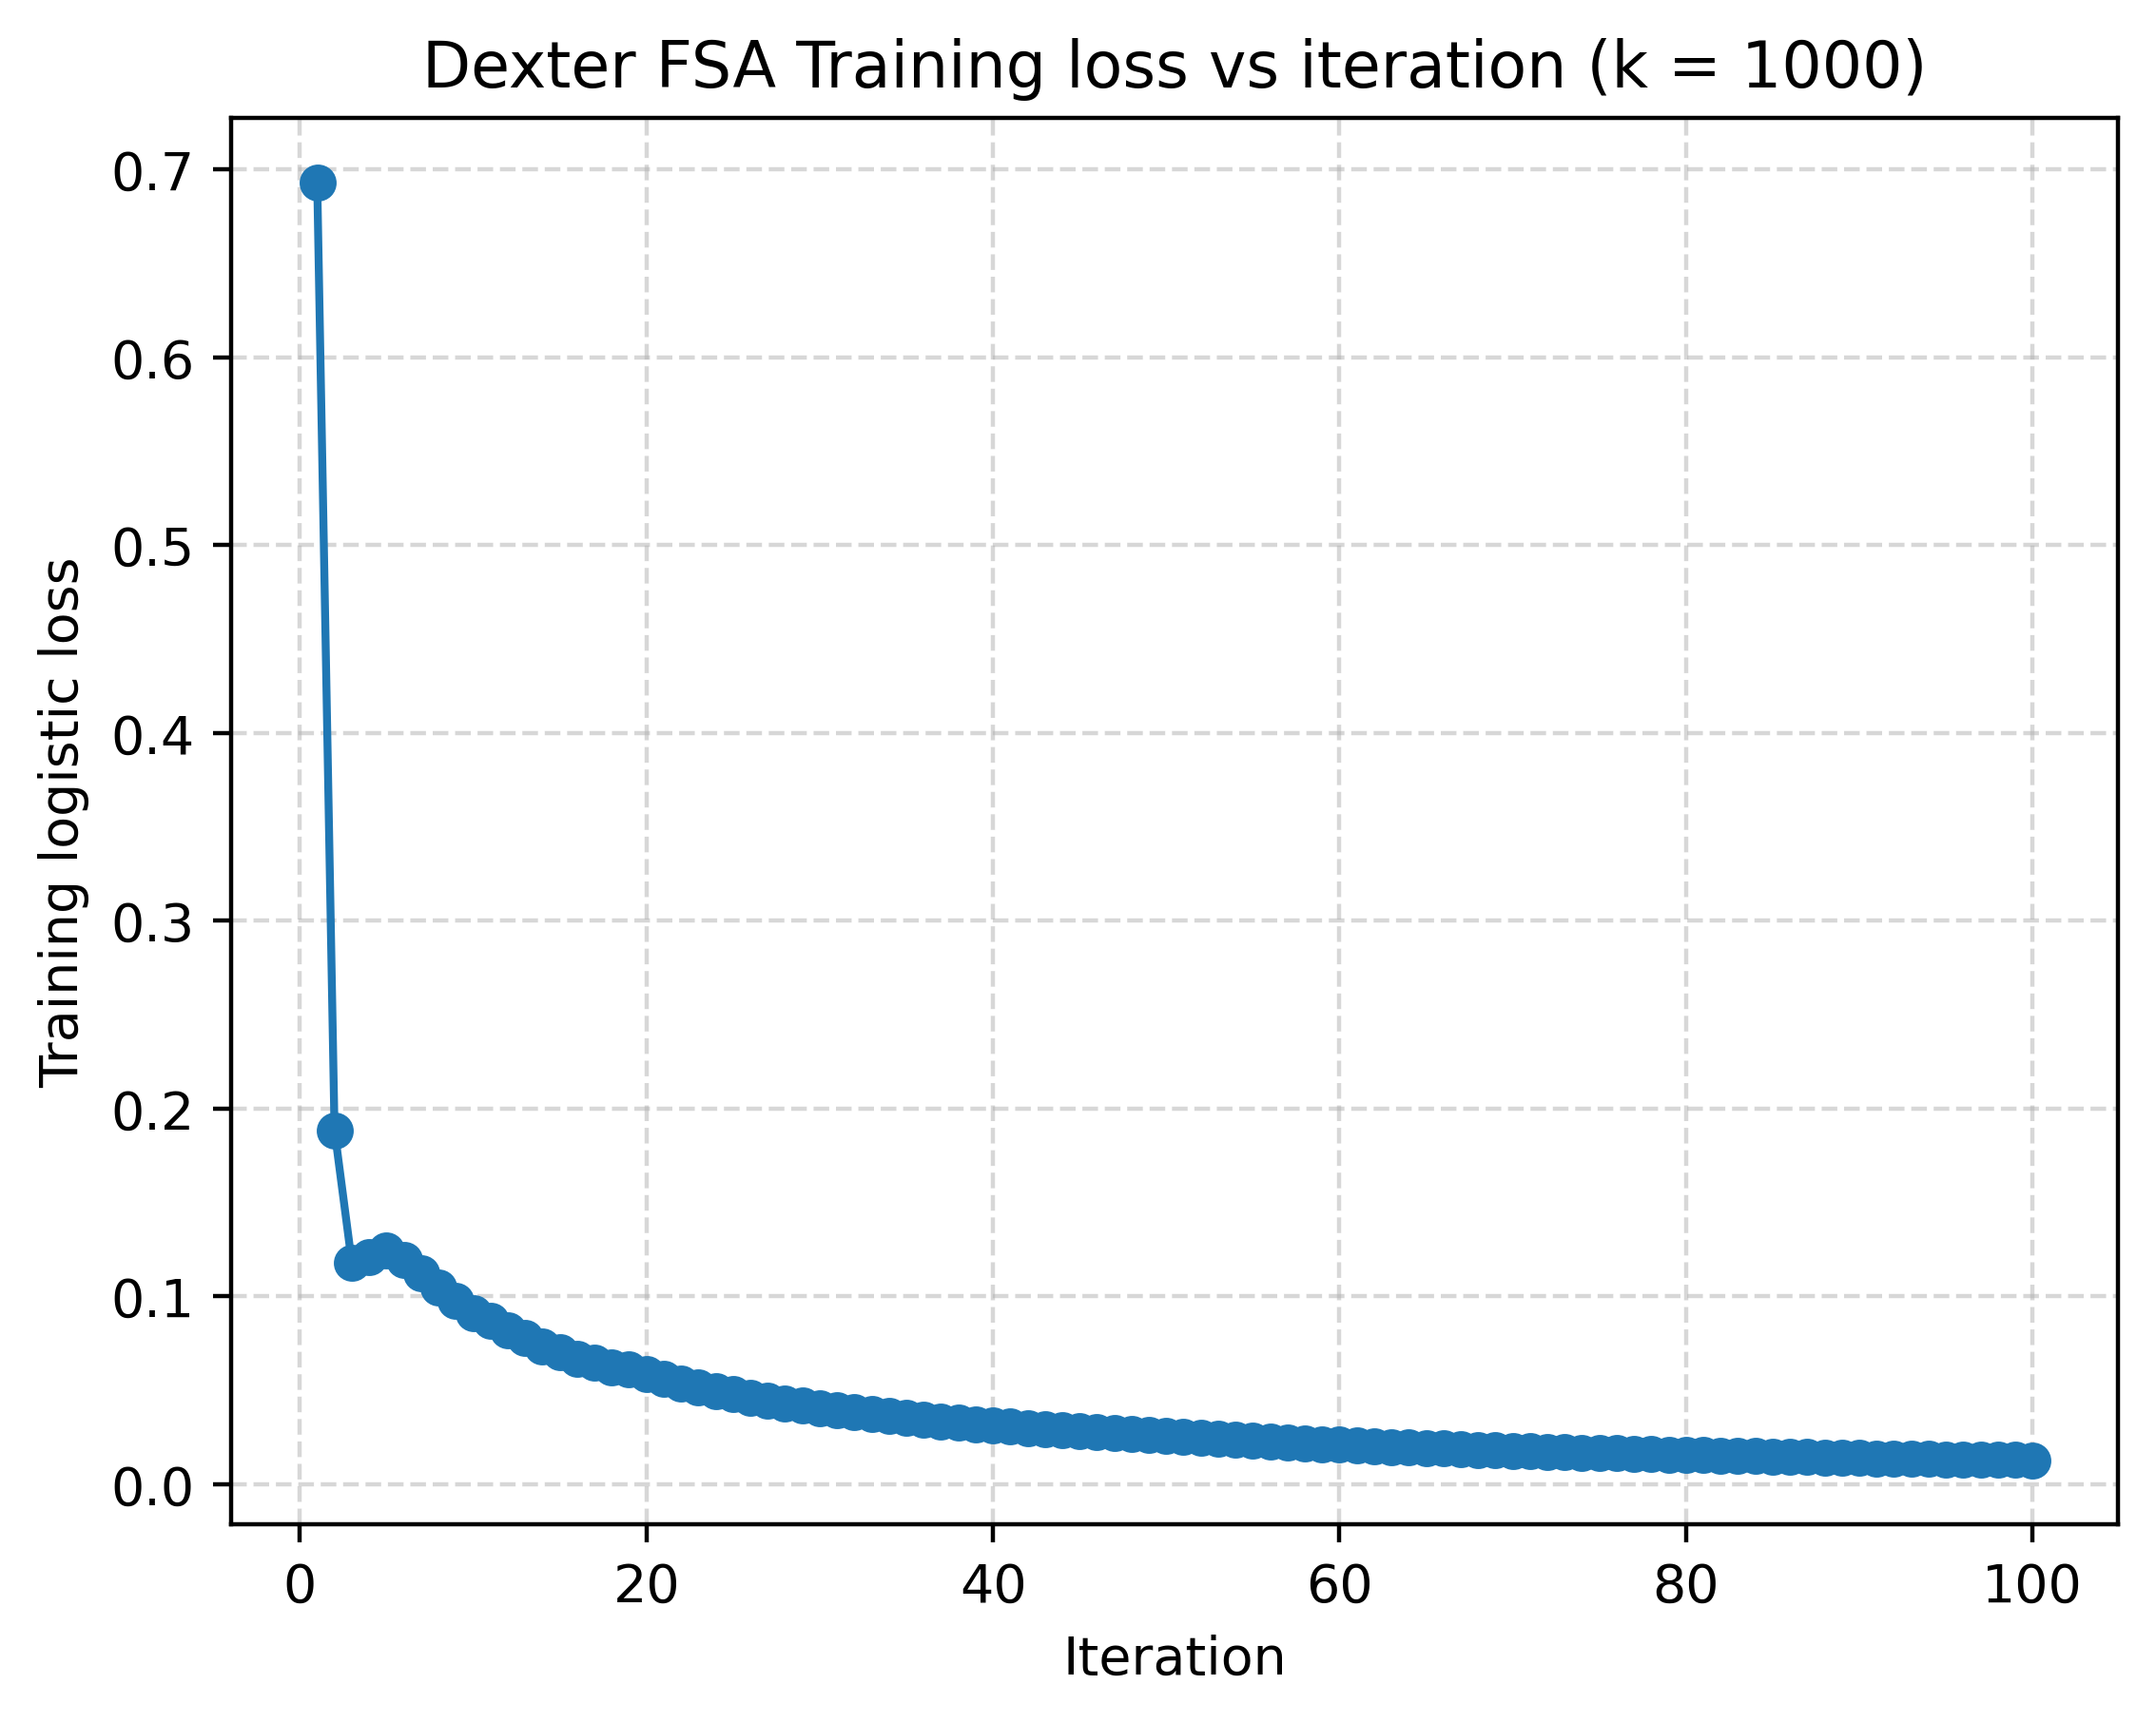
\includegraphics[width=\linewidth]{../figures/dexter_misclass_1000_FSA.png}
        \caption{Dexter Dataset}
    \end{subfigure}
    \caption{Plot of Training Loss vs. Iteration Number for \(k=1000\).  Gisette Dataset (left), Dexter
    Dataset (right).}
    \label{fig:q2}
\end{figure}
At first glance, neither datasets training loss converges, which makes sense.  \(\mu\) is only 100 and
we only have 100 iterations; \(\mu\) is usually 300 and we typically have more iterations.  

The table reporting train and test misclassification errors, test AUC, and training time is shown in 
Table \ref{tab:table_q2}:

 \begin{table}[htbp]
    \centering
    \resizebox{\textwidth}{!}{
        \input{../output/misclass_table_q2.tex}
    }
    \caption{Train and Test Misclassification Errors, Test AUC, and training time, FSA algorithm.}
    \label{tab:table_q2}
\end{table}

\end{document}